\section{MTU Discovery}
\label{sec:MTU Discovery}

\subsection{Einleitung}
Mithilfe der \acs{MTU} (Maximum Transmission Unit) wird festgelegt wie gross ein Netzwerkpaket maximal sein darf, so dass es nicht in mehrere Pakete aufgeteilt werden muss. Wenn die \acs{MTU} korrekt bestimmt wurde dann wird Paket-Fragmentierung verhindert und die Performance der Netzwerkverbindung ist deutlich besser. 

\subsection{Path MTU Discovery}
Normalerweise wird die \acs{MTU} automatisch via \acs{PMTUD} (Path MTU Discovery) ermittelt. Dabei werden \acs{ICMP} Pakete unterschiedlicher Grösse die mit einem \enquote{Don't fragment} Flag versehen sind über die Verbindung gesandt. Wenn ein solches Paket auf ein Netzwerkgerät trifft dass eine kleinere \acs{MTU} konfiguriert hat als die Paketgrösse wird das Paket nicht weitergesendet, stattdessen wird ein \acs{ICMP} Paket mit dem Inhalt "Fragmentation needed" retourniert. So weiss der \acs{PMTUD} Algorithmus dass die \acs{MTU} der Verbindung überschritten wurde \cite[:131]{rfc1191}.

\acs{PMTUD} hat jedoch ein Problem. Router die, die \acs{ICMP} Pakete weiterleiten oder aber ein \enquote{Fragmentation needed} Paket zurücksenden sollten tun dies nicht immer. Dieses Fehlverhalten gibt es aus mehreren Gründen. Zum einen wegen Kernel-Bugs, Fehlkonfigurationen und zum anderen auch weil Firewalls manchmal so konfiguriert werden dass sie \acs{ICMP} Nachrichten nicht durchlassen auf Grund von Sicherheitsbedenken \cite[:137]{rfc2923}.

Da man sich also nicht auf \acs{PMTUD} verlassen kann um die \acs{MTU} einer Verbindung festzustellen wird mit dieser Arbeit eine \acs{MTU} Discovery implementiert die innerhalb einer \acs{IPSec} \acs{VPN} Verbindung durchgeführt werden kann.

\subsection{MTU Discovery innerhalb des Tunnels}
Um die im vorherigen Kapitel erwähnten Probleme von \acs{PMTUD} zu vermeiden wird die \acs{MTU} vom im \tool implementierten Algorithmus innerhalb des \acs{VPN} Tunnels festgestellt.

Dazu werden \acs{ICMP} Pakete vom Typ \enquote{ICMPv4TypeEchoRequest} und \enquote{ICMPv4TypeEchoReply} verwendet. Diese Pakete werden wie bei \acs{PMTUD} mit einem \enquote{Don't fragment} Flag versehen. Im Unterschied zu \acs{PMTUD} werden sie aber innerhalb des \acs{VPN} Tunnels verschickt und werden daher in \acs{ESP}s gekapselt. Ausserhalb des Tunnels sind sie so nicht unterscheidbar vom normalen Verkehrs des Tunnels und können daher nicht blockiert werden. Der \enquote{Don't fragment} Flag wird aber bis in die \acs{ESP} Hülle weitergezogen so dass auch das \acs{ESP} welches das \acs{ICMP} Paket transportiert nicht fragmentiert wird.

\todo{Screenshot Ausschnitt das ESP mit \enquote{Don't fragment} flag zeigt.}

Um den \acs{MTU} Discovery Vorgang zu starten wird jeweils ein \enquote{ICMPv4TypeEchoRequest} versendet. Wenn auf dem Ziel Computer Ping Replys aktiviert sind dann löst dieses Paket eine automatische Antwort aus die mit dem gleichen Paketinhalt zurückgeschickt wird. Wenn Ping Replys nicht aktiviert sind kann auch das \tool diese Arbeit übernehmen und eine passende Antwort zurückschicken.

Alle vom \tool verschickten \acs{ICMP} Pakete haben jeweils die folgende Payload:

\begin{itemize}
  \item \textbf{AppID:} Eindeutige ID des aktiven \tool. Wird verwendet um mehrere gleichzeitig laufende \tool auf einem Rechner zu unterscheiden. Die AppID wird entweder in der Konfiguration fix festgelegt oder auf 0 gesetzt. Wenn die AppID in der Konfiguration auf 0 gesetzt wurde dann wird beim Programmstart eine zufällige AppID generiert.
  \item \textbf{ChannelID:} ID des GO-Channels von dem das Paket versendet wurde. Wird benötigt um für mehrere Tunnels gleichzeitig die \acs{MTU} festzustellen zu können. Die ChannelID wird jeweils beim Start eines \acs{MTU} Discovery Vorgangs zugeteilt.
  \item \textbf{Command:} Die eigentliche Nachricht des Pakets. Wird verwendet um sicherzustellen dass dieses \acs{ICMP} Paket wirklich von einem \tool versendet wurde und nicht ein sonstiges \acs{ICMP} Paket.
  \item \textbf{Null-Array:} Ein mit Nullen gefülltes Array von variabler Grösse. Wird verwendet um dem Paket seine vorbestimmte Grösse zu geben.
\end{itemize}

% GFX Trim left bottom right top
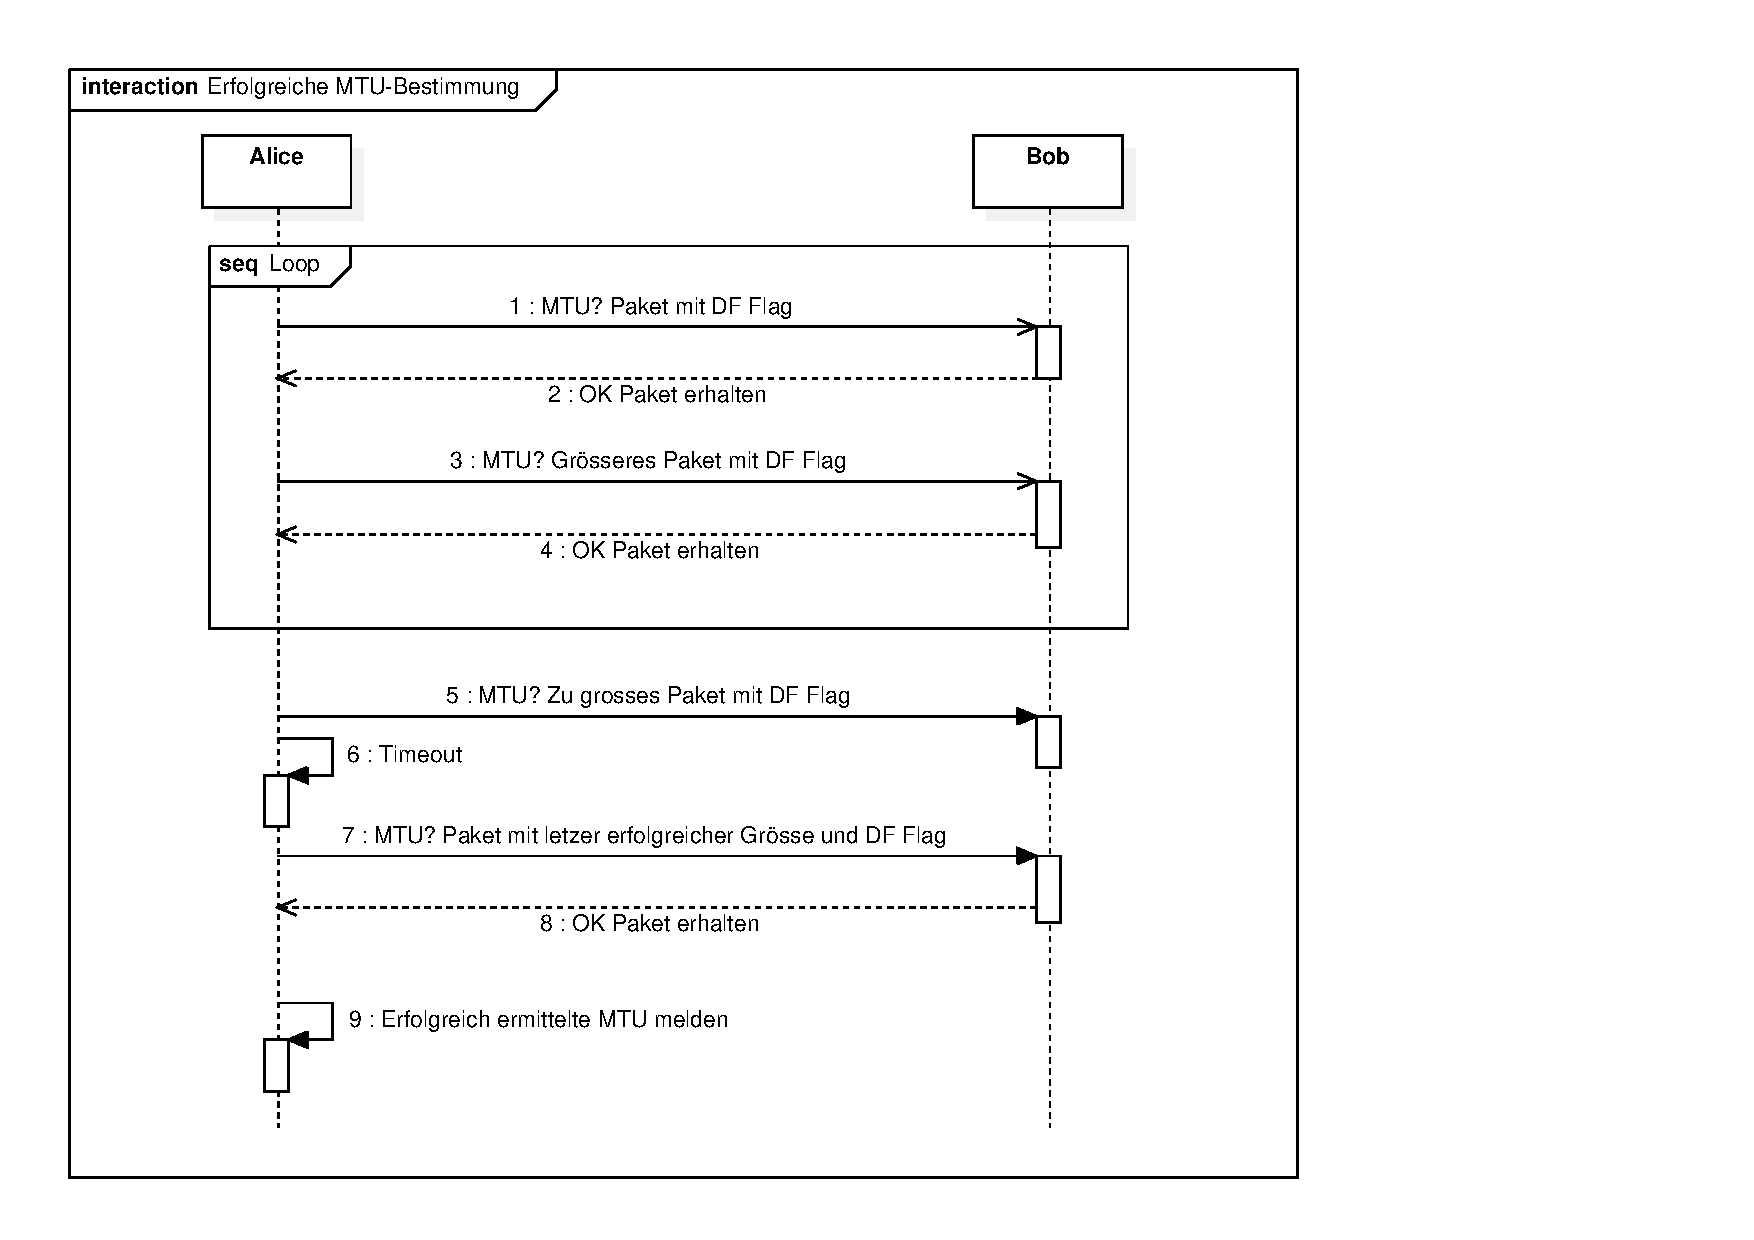
\includegraphics[trim=10 10 200 10,clip,width=\textwidth]{mainpart/implementation/img/MTUBestimmungErfolgreich}

Die obenstehende Grafik zeigt den weiteren Ablauf der \acs{MTU} Bestimmung mit dem \tool. Alice sendet ein Paket mit dem Command \enquote{MTU?} und einer bestimmten Grösse an Bob. Wenn Bob das Paket erhält, sendet er "OK als Antwort. Alice erhöht darauf die Paketgrösse und fragt Bob erneut mit "MTU?" an. Dies wird so lange wiederholt bis das Paket nicht mehr ankommt. Bob erhält also das "MTU?" Paket nicht und kann somit Alice auch keine Antwort schicken. Alice hat jedoch ein Timeout Timer und nach einer vordefinierten Zeit ohne Antwort geht Alice davon aus dass das Paket nicht angekommen ist. Alice sendet nun ein Paket mit der letzten erfolgreichen Grösse um sicher zu Stellen das die Netzwerkverbindung selbst noch besteht und protokolliert dann die letzte erfolgreiche \acs{MTU}.

\subsection{MTU-Bestimmung - FastMTU}
Die im oberen Abschnitt beschrieben Art der \acs{MTU} Bestimmung war gut als ein erster Schritt im iterativen Softwareentwicklungsprozess. Für einen produktiven Betrieb wäre sie aber nicht zu gebrauchen. Zum einen ist die oben beschriebene Variante nur exakt wenn man einen Vergösserungs-Schritt von einem Byte nimmt und wodurch der Algorithmus aber sehr langsam wird. Und zum anderen ist sie auch Anfällig auf Paket-Verluste.
Daher wurde der Algorithmus nach der ersten Iteration erweitert und überarbeitet. Die neue Variante wird von uns liebevoll "FastMTU" genannt.

Bei der FastMTU Bestimmung bleibt das grundlegende Prinzip gleich, es werden Pakete unterschiedlicher Grösse versendet so dass man herausfinden kann welche ankommen und welche verworfen werden. Neu wird jedoch nicht nur ein Paket aufs Mal versendet sondert einen ganze Batch von Paketen. Dazu wird aus der Konfiguration einen sogenannten Range ausgelesen. Der Range besteht aus zwei Byte-Grössen die festlegen worin sich die \acs{MTU} typischerweise befinden sollte. Zum Beispiel zwischen 0 und 2000 Bytes. Dann wird aus der Konfiguration ausgelesen wie viele Pakete aufs Mal versendet werden sollen. Mehr gleichzeitige Pakete führen zu einer schnelleren Bestimmung der \acs{MTU}, haben aber auch zur folge dass die Verbindung stärker belastet wird und so möglicherweise wichtiger Kunden-Traffic ausgebremst wird. Als Default-Wert gehen wir von 20 gleichzeitigen Paketen aus. Der Range 0-2000 Bytes wird jetzt also durch 20 geteilt. Damit erhält man 20 Pakete die sich je um 100 Bytes unterscheiden. Diese 20 Pakete werden nun als einen Batch versendet.
Für alle Pakete die auf der anderen Seite des Tunnels ankommen wird nun eine Antwort generiert. Bei einer MTU von 1500 Bytes würden die ersten 15 Pakete ankommen. Der Sender weiss jetzt also dass die exakte \acs{MTU} zwischen dem letzten erfolgreichen Paket (1500) und dem ersten nicht erfolgreichen Paket (1600) sein muss. 1500-1600 Bytes wird nun als nun als neuer Range gesetzt und erneut durch die Anzahl gleichzeitiger Pakete geteilt. Die Pakete des zweiten Batches haben also noch 5 Byte Unterschied. Dieser Vorgang wird so lange wiederholt bis der Unterschied zwischen den Paketen eines Batches nur noch 1 Byte sind. Jetzt weiss man das man die exakte \acs{MTU} gefunden hat.

Mit FastMTU weiss man also bereits im vorraus wie lange das Finden der exakten \acs{MTU} dauern wird. Bei einer MTU zwischen 0-2000 Bytes werden 3 Batches an Paketen versendet. Pro Batch muss jeweils die Dauer des Timeout-Timers gewartet werden. Gemäss der \osag ist ein Timeout von 10 Sekunden realistisch. Daher hätte das Bestimmen diese \acs{MTU} 30Sekunden gedauert.
Die verbrauchte Zeit beim Bestimmen von FastMTU lässt sich sehr leicht via der Konfiguration optimieren. So hat man die Möglichkeit den Range stärker einzuschränken, den Timeout zu verkürzen oder aber mehr Pakete pro Batch zu versenden.

\todo{Grafik die FastMTU zeigt.}

Auch wenn die \acs{MTU} sich ausserhalb des Ranges befindet wird sie von FastMTU noch korrekt detektiert. Wenn nämlich alle Pakete eines Batches eine erfolgreiche Antwort der Gegenseite generieren, dann wird der nächste Range einfach um die Grösse des überprüften Range vergrössert. Im Beispiel mit einem Range von 0-2000 Bytes würde jetzt einfach 2000-4000 Bytes überprüft.